\documentclass[11pt,letterpaper]{article}

%% Language and font encodings
\usepackage[english]{babel}
\usepackage[utf8x]{inputenc}
\usepackage{comment}
\usepackage{booktabs}
\usepackage{tabu}
\usepackage{bbm} %Indicator function
\usepackage[T1]{fontenc}
\usepackage{multirow}
%% Sets page size and margins
\usepackage[letterpaper,top=1in,bottom=1in,left=1in,right=1in]{geometry}

%% Useful packages

\usepackage{amsmath}
\usepackage{amssymb}
\usepackage{amsthm}
\usepackage{graphicx}
\usepackage[colorinlistoftodos]{todonotes}
\usepackage[colorlinks=true, allcolors=blue]{hyperref}
\usepackage{apacite}
\RequirePackage{import} %-> Import files from other folders
\usepackage{float} %-> Table and figure positioning
\usepackage{footmisc}%Footnote symbols package
\usepackage{cancel}
\hypersetup{
  bookmarksnumbered,
  bookmarksopen,
  bookmarksopenlevel=0,
  colorlinks,
% for colors, check package xcolor
%   anchorcolor=anchorcolor,
    citecolor=blue,
%   linkcolor=linkcolor,
	pdfauthor={Rodrigo Azuero Melo},
	pdftitle={Evaluating Early Childhood Interventions},
	pdfsubject={},
	pdfkeywords={},
%   plainpages=false,
%   urlcolor=urlcolor
}

\title{Class 2}
\author{Doc author: \href{mailto:razuero@iadb.org}{razuero@iadb.org}}
\date{December 2018}

\begin{document}
\maketitle
In this section we will cover, some basics of R, a review of Ordinary Least Squares (OLS), and maximum likelihoood estimation.



\section{R Basics}
R is a programming language and a software environment. It is free, with an active community developing packages and improvements continuously. The purpose of this tutorial is not to cover all the features of R but rather to give you a basic understanding of the programming language and some novel things you can do with this software. 
\subsection{Installing R}
You will need to install R and Rstudio. Rstudio is an integrated development environment (IDE) for the programming language R. 
\begin{enumerate}
    \item Install R from \href{https://cran.r-project.org/}{https://cran.r-project.org}
    \item Install R Studio from \href{https://www.rstudio.com/products/rstudio/download/}{https://www.rstudio.com/products/rstudio/download/}
\end{enumerate}
Once you have installed R and Rstudio, you are ready to run some code. The first thing we will do is install some packages we will use for our introductory class. 'data.table' is a package commonly used for data handling. We will install it and learn the basics of how to use it. You can find more information with examples about the package `data.table' in \href{https://cran.r-project.org/web/packages/data.table/vignettes/datatable-intro.html}{this link}.

\begin{verbatim}
    >install.packages('data.table')
    >library(data.table)
\end{verbatim}

Now we will open a dataset containing information about wages, years of schooling, and age of 800 individuals:
\begin{verbatim}
    >WageD<-read.table("https://raw.githubusercontent.com/rodazuero/samplecode
    /master/CUDA/mle_mincer/DATACUDA.csv",sep = ",")
    >WageD<-data.table(WageD)
\end{verbatim}

Assigning the names to the WageD dataset:
\begin{verbatim}
    colnames(WageD)<-c(`age',`schooling',`logwage')
\end{verbatim}

and we are ready to start with some calculations and graph with the data. Let's compute the averages and standard deviations of our series:
\begin{verbatim}
    >mean(WageD$exp(logwage))
    >sd(WageD$exp(logwage))
    
    >mean(WageD$age)
    >sd(WageD$age)
    
    >mean(WageD$schooling)
    >sd(WageD$schooling)
\end{verbatim}

Let's say we are interested in the median wages of people who have higher education and are under 50 years of age. How can we do this with `data.frame'?

\begin{verbatim}
    >mean(exp(WageD[age < 50 & schooling > 12]$logwage))
\end{verbatim}

[{\color{red}recall $mean(exp(X))\neq exp(mean(X))$]. Jensen's inequality }
\\
Let's plot some relationships in the data. For this, we will use the package ggplot, which is one of the most popular packages for data visualization in R. You can find more resources about ggplot in \href{https://ggplot2.tidyverse.org/}{this link}.

\begin{verbatim}
    >install.packages(`ggplot2')
    >library(ggplot2)
    >p <- ggplot(WageD, aes(logwage, schooling))
    >p<-p + geom_point()
    >p
\end{verbatim}

The result is presented in Figure \ref{fig:logwagedu}
\begin{figure}[H]
\begin{center}
\caption{Relationship between log-wages and schooling}
\label{fig:logwagedu}
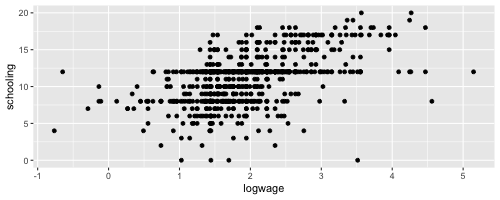
\includegraphics[width=0.8\textwidth]{LogWageSchooling.png}
\end{center}
\end{figure}
Try to plot the relationship with exp(logwage), the actual wage, and see the differences in the relationship. Now, let's say we want to analyze the relationship between schooling and wages for people who are under 40 and those who are over 40.

\begin{verbatim}
    >WageD$agegroup = cut(WageD$age,c(0,40,100))
    >sizeT=1.5
    >p <- ggplot(WageD, aes(logwage, schooling))
    >p<- p+ geom_point(aes(colour = factor(agegroup)))
    >p<-p + theme(
        plot.title = element_text(size = rel(sizeT)),
        axis.title=element_text(size = rel(sizeT)),
        axis.text.x=element_text(size = rel(sizeT)),
        axis.text.y=element_text(size = rel(sizeT)),
        legend.text=element_text(size = rel(sizeT)),
        panel.background = element_rect(fill="grey96"),
        legend.key=element_blank(),
        legend.title=element_blank())
    >p<-p+xlab("log(wages)")
    >p<-p+ylab("years of schooling")
\end{verbatim}

\begin{figure}[H]
\begin{center}
\caption{Relationship between log-wages and schooling by age groups}
\label{fig:logwagedugroups}
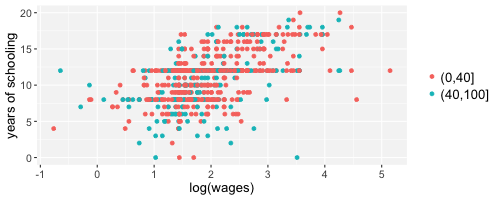
\includegraphics[width=0.8\textwidth]{LogWageSchoolingGroup.png}
\end{center}
\end{figure}




\section{OLS Basics}
The goal of OLS is to fit a linear function to the data by minimizing the sum of squared errors. Suppose we have data on log-wages, denoted by $y_i$, for $n$ individuals:
\begin{equation}
    Y_{n\times 1}=\begin{bmatrix} y_1\\ y_2 \\ \vdots \\ y_n \end{bmatrix}
\end{equation}
We also have information on individuals' years of schooling $(X_1)_{n\times1}$ and age $(X_2)_{n\times1}$ and we want to analyze the relationship between education, age, and wages. For each individual, our predicted wage  will be:
\begin{equation}
    \hat y_i=\beta_0+\beta_1x_{1,i}+\beta_2 x_{2,i}
\end{equation}
The goal in OLS is to minimize the sum of squared errors. That is, we want to find $\beta_0,\beta_1,\beta_2$ that minimize the following loss function defined in Equation \ref{eq:lossOls}
\begin{align}\label{eq:lossOls}
    L(\beta_0,\beta_1,\beta_2;Y,X_1,X_2)= & \sum_{i=1}^n\left(y_i-\hat y_i\right)^2\nonumber \\[0.2in]
    & = \sum_{i=1}^n\left(y_i-\beta_0-\beta_1x_{1,i}-\beta_2 x_{2,i}\right)^2
\end{align}
We will skip the derivation of the parameters $\beta_0,\beta_1,\beta_2$\footnote{If you are interested in the derivation you can check various textbooks. The Wikipedia entry includes some derivations} but it can be shown that:
\begin{align}
    \beta=\left(X'X\right)^{-1}\left(X'Y\right)
\end{align}
where:
\begin{align}
    X_{n\times 3}=\begin{bmatrix}X_0,X_1,X_2\end{bmatrix}
\end{align}
\begin{align}
    (X_0)_{n\times 1}=\begin{bmatrix}1\\ 1\\ \vdots \\1\end{bmatrix}
\end{align}
\begin{align}
    \beta=\left[\beta_0,\beta_1,\beta_2\right]
\end{align}

\subsection{Code your own OLS}
Now that we know the basics of R programming language and how to derive the coefficient estimates for OLS, we will code our own OLS function. 

\begin{verbatim}
    n<-length(WageD$logwage)
    X0<-rep(1,n)
    X1<-WageD$age
    X2<-WageD$schooling
    Y<-WageD$logwage


    X<-cbind(X0,X1,X2)

    Beta<-(solve(t(X)%*%X))%*%(t(X)%*%Y)
    Beta0<-Beta[1]
    Beta1<-Beta[2]
    Beta2<-Beta[3]
\end{verbatim}

Compare your results with the coefficients obtained directly from the $lm$ function in R. We will not go through the derivation of the standard errors of the linear regression model. 
\begin{verbatim}
    >mod<-lm(logwage~ age+schooling, WageD)
    >print(coef(summary(mod)))
    
             Estimate     Std. Error   t value   Pr(>|t|)
(Intercept) 0.343963408 0.137502893  2.501499 1.256636e-02
age         0.007880537 0.002932586  2.687231 7.354874e-03
schooling   0.116905614 0.006881529 16.988321 1.792663e-55

\end{verbatim}

\subsection{Code your own OLS advanced}
Now we will code our own OLS finding the coefficients that minimize a function that we will create which is the sum of squared errors.

\begin{verbatim}
    >SSR<-function(Beta){
    >Pred<-Beta[1]+Beta[2]*WageD$age+Beta[3]*WageD$schooling
    >SR<-(WageD$logwage-Pred)^2
    >ans<-sum(SR)
    >return(ans)
    >}

    >BetaInic<-c(1,1,1)
    >Parameters<-optim(BetaInic,SSR)
    >Parameters$par

\end{verbatim}
How does your own estimates of $\beta$ compare with the ones of $lm$?
\section{MLE}
Suppose the data $\{Data\}_{i=1}^n=\{Wage,age,schooling\}_{i=1}^n$ has a density $f(Data;\Theta)$. The density $f(.)$ is known up to a parameter $\Theta$. The joint density is given by $\bar f:$
\begin{align}
    \bar f(Data_1,Data_2,....,Data_n;\Theta)
\end{align}
If the data is i.i.d, the joint density can be written as the product of independent pdf's:
\begin{align}
    \bar f(Data_1,Data_2,....,Data_n;\Theta)=
    f(Data_1;\Theta)\times f(Data_2;\Theta),...,f(Data_n;\Theta)
\end{align}
The likelihood function is the joint pdf but it is considered a function of the parameter $\Theta$ conditional on the data:
\begin{align}
    \mathcal{L}(\Theta,Data)=\prod_{i=1}^nf(Data_i;\Theta)
\end{align}
\textbf{Caution:} you cannot interpret the likelihood as the probability of observing the dataset conditional on a parameter. In continuous random variables the pdf is not the probability. 
\\
Let's assume that log-wages are determined according to the following model:
\begin{align}\label{eq:individuallikelihood}
    \text{logwage}_i=\beta_0+\beta_1\text{age}_i+\beta_2\text{yrschool}_i+\varepsilon_i
\end{align}
And consider the case where
\begin{align}
    \varepsilon_i\sim \mathcal{N}(0,\sigma^2)
\end{align}
Recall, the pdf of random variable $x$ following a normal distribution with mean $\mu$ and variance $\sigma^2$ is:
\begin{align}
    \phi(x;\mu,\sigma^2)=\frac{1}{\sqrt{2\pi \sigma^2}}e^{-\frac{1}{\sigma^2}\left(x-\mu\right)^2}
\end{align}
From Equation \ref{eq:individuallikelihood} we see that the pdf of logwages follows the distribution described in Equation \ref{eq:likelihood2}:
\begin{align}\label{eq:likelihood2}
    f(\text{logwage}_i;\text{age,yrschool,}\sigma^2)=\mathcal{N}\left(\beta_0+\beta_1\text{age}_i+\beta_2\text{yrschool}_i,\sigma^2\right)
\end{align}
Then the joint likelihood becomes:
\begin{align}
    \mathcal{L}(\Theta;Data)=\prod_{i=1}^n(f(\text{logwage})_i;\beta,\sigma^2)
\end{align}
Likelihood functions are usually very close to zero. For computational precission, we usually work with the log-likelihood function. 
\begin{align}
    l(\Theta;Data)= & \ln\left(\mathcal{L}(\Theta;Data)\right)\nonumber \\[0.2in]
    & = \sum_{i=1}^nln(f(\text{logwage})_i;\beta,\sigma^2)
\end{align}
where all the parameters $\Theta=\left[\beta_0,\beta_1,\beta_2,\sigma^2 \right]$

The maximum likelihood estimator: $\Theta_{\text{MLE}}=\left[\beta_0,\beta_1,\beta_2,\sigma^2\right]$ is:
\begin{align}\label{eq:lastmle}
    \Theta_{\text{MLE}}=\arg max_{\Theta} l(\Theta;Data)
\end{align}


\subsection{MLE in R}
In this section we will compute the Maximum Likelihood estimators of the model described in Equations \ref{eq:individuallikelihood} - \ref{eq:lastmle}. First, we define the likelihood function of each individual observation. This is an intuitive, but computationally slow, way of defining the likelihood function
\begin{verbatim}
Likelihood<-function(Theta){
  bbeta0<-Theta[1]
  bbeta1<-Theta[2]
  bbeta2<-Theta[3]
  ssigma<-exp(Theta[4])
  
  loglik=0;
  for(i in 1:n){
    predlogwage<-bbeta0+bbeta1*WageD$age[i]+bbeta2*WageD$schooling[i]
    yobserved<-WageD$logwage[i]
    error<-yobserved-predlogwage
    loglikelihood=log(dnorm(error,mean=0,sd=(ssigma)))
    loglik=loglik+loglikelihood
  }
  loglik=-loglik
  print(loglik)
  return(loglik)
  
}
\end{verbatim}

Once defined the (negative) of the likelihood function, we find the parameters that maximize (minimize the negative):
\begin{verbatim}
    >Theta<-c(1,1,1,1)
    >Likelihood(Theta)
    >Parameters<-optim(Theta,Likelihood)
    >Parameters
\end{verbatim}


How does your estimates of ML compare to OLS? 

\section{Advanced topics}
Some topics we can discuss if time allows:
\begin{enumerate}
    \item \textbf{Large sample properties}. Consistency, efficiency of OLS and MLE.
    \begin{itemize}
    \item What is consistency? Consistency and unbiasedness.
    \item What is efficiency?
    \item Assumptions for unbiasedness and consistency of OLS estimator. 
    \item Consistency and efficiency of OLS and MLE: Both estimators are consistent EVEN if real distribution of $\varepsilon$ is not $\mathcal{N}$. MLE is efficient under right specification. Heteroskedasticity, etc. 
    \end{itemize}
    \item \textbf{Parallelization}. This is a topic that I think we should addres at least in the neural networks part. GPU parallelization is the standard way of estimating neural networks and, although we won't expect people to run their own cuda routine, at least to know what it is. Although we can go more into the details on the NN class, I provide an example of parallel computation of the likliehood function of the model introduced.  \href{https://www.analyticsvidhya.com/blog/2017/05/gpus-necessary-for-deep-learning/}{https://www.analyticsvidhya.com/blog/2017/05/gpus-necessary-for-deep-learning/}
    \begin{itemize}
        \item Moore's law and why we need parallelization
        \item Parallelization: basics. 
        \item GPU vs CPU parallelization
        \item Estimate maximum likelihood function of the model mentioned before via parallelization through the GPU. \href{https://github.com/rodazuero/samplecode/blob/master/CUDA/mle_mincer/CUDAMLE.cu}{see link}
    \end{itemize}
    \item \textbf{Advanced R}. Let's discuss something else you can do in R
    \begin{itemize}
        \item web-scrape
        \item shiny
        \item etc. 
    \end{itemize}
\end{enumerate}





\end{document}